% Command to multiply a variale by a floating point number.
\newcommand*{\Mul}[2]
{
  \FPeval{vTemp}{#1 * #2}
  \FPround\vTemp{\vTemp}{4}  % Round to four digits after decimal point.
  \FPprint{vTemp}
}

% Command to print the result #1 / #2.
\newcommand*{\Div}[2]
{
  \FPeval{vTemp}{#1 / #2}
  \FPround\vTemp{\vTemp}{4}  % Round to four digits after decimal point.
  \FPprint{vTemp}
}

\documentclass{article}
\usepackage[nomessages]{fp}  % http://ctan.org/pkg/fp
\usepackage[pdftex]{graphicx}
\usepackage{gensymb}
\usepackage[T2A]{fontenc}
\usepackage[utf8]{inputenc}
\usepackage[bulgarian]{babel}
\usepackage[table]{xcolor}     % For coloured rows within tables.
\usepackage{siunitx}
\usepackage{systeme}
\usepackage{amsfonts}  % For set symbols e.g. N, R, C etc.
\usepackage{mathtools}

% Not sure if siunitx includes this, so defining it myself.
\DeclareSIUnit{\rpm}{ rpm}

\begin{document}

\begin{titlepage}
\begin{center}
\textsc{\Large Manufactoring Desing II Coursework}\\[1cm]
\textsc{\Huge Gearbox for Machining Center}\\[1.5cm]
\textsc{\Large Miroslav Vitkov}\\[0.5cm]
\textsc{Faculty number: 221207005}\\[1.5cm]
% TODO: include image of final design
\vfill
\today
\end{center}
\end{titlepage}

\section{Requirements}
Design a 2-speed gearbox for a vertical machining center.
The speeds needn't be changed at running motor. \\
$$P_{output, max} = 11 \si{\kilo\watt}$$
$$n_{output, max} = 5000 \si{\rpm}$$

\section{Motor selection}
From [4] we select the Siemens 1PH209 spindle motor.
It is the recommended built-in motor for standard machine tool spindle.
Outside diameter is 205 mm, output shaft diameter 67 mm.
Nominal speed 1500 rpm, maximum 10000 rpm.
As the motor can be requested in different power ratings, we purchase one for 12kW as to compensate frcition losses.
\\
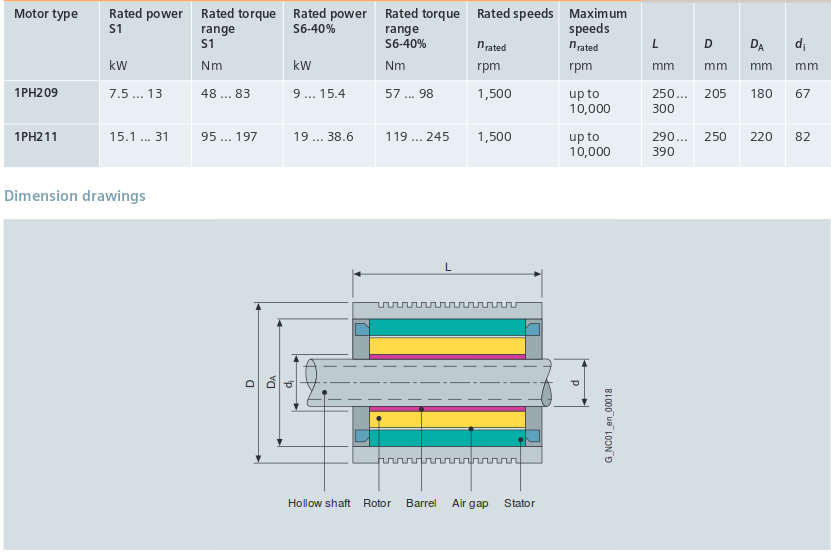
\includegraphics[width=1.25\textwidth]{images/motor}~

\section{Kinematic diagram} % (plan for rotational velocities)
The goal of the gearbox is to provide sufficient torque to the spindle at low motor speeds (below $n_{nominal}$).
For selecting the low gear we utilize the rule of thumb to choose a transfer ratio between $1/3$ and $1/4$:
$$ TR_1 = 1/4 $$
For selecting the high gear, we try to match the maximum speed of the motor with the required maximum spindle speed by specification:
$$ TR_2 = n_{spindle, max} / n_{motor, max} = 5000 / 10000 = 1/2$$
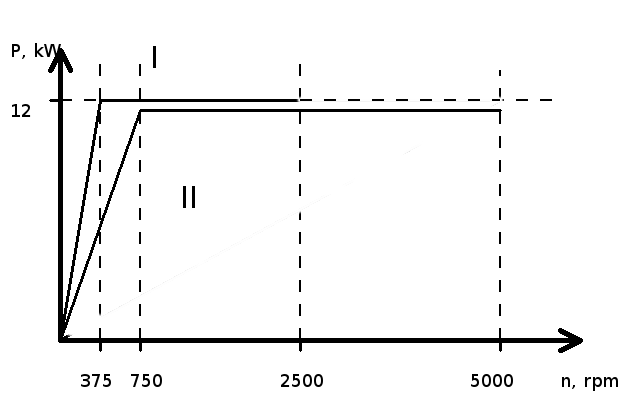
\includegraphics[width=0.75\textwidth]{images/kinematics}~

\section{Components sizing}
\subsection{Gears}
Requirements: Design input shaft gears G11 and G12 and output shaft gears G21 and G22
Both center distances (G11-G21 and G12-G22) must be equal.
All gears must be capable of transmitting the rated power at all speeds..
Gear teeth must be shaped with a cutoff or round-off to assist gear engagement.  % зъбозаобляне
Conventional spur gears with involute teeth profile have been selected for this application.
\subsubsection{Standard Basic Rack Tooth Profile}
Due to the numerous advantages of using standard tooth geometry, we decide to adhare to the Standard Basic Rack Tooth Profile [5]. \\
Pressure angle: $\alpha = 20\degree$  \\
Addendum circle: $h_a = 1.00m$ \\
Bottom clearance: $c = 0.25m$ \\
Daedendum circle: $h_f = 1.25m$ \\
Fillet radius: $\rho = 0.38m$ \\
Active tooth depth: $h_w = 2.00m$ \\
Whole depth: $h = 2.25m$ \\
Tooth thickness: $s = (\pi m)/ 2$ \\
\\
From [6] we select standard module and number of teeth for G11.
The module is limitted to be select among the standard modules[6]: $1, 1.25, 1.5, 2, 2.5, 3, 4, 5, 6, 8, 10$ etc.
The number of teeth on the pinion is limitted by $z_{min} = 17$ and $z_{max} = 33$ [6]. \\
$$m_{11} = 6 \si{\milli\meter}$$
$$z_{11} = 17$$
Now calculate G21, meshing with G11.
For a transfer ratio of $TR_1 = 0.25$, we would need G21 to have number of teeth: \\
$$ z_{21} = z_{11} / TR_1 = 17 / 0.25 = 68 $$
$$ m_{21} = 6\si{\milli\meter}  $$
This results in a center distance for G11-G21 of: \\
$$ a_1 = \frac{d_1 + d_2}{2} = \frac{m_{11} z_{11} + m_{21} z_{21}}{2} = 255 \si{\milli\meter}$$
Now we need to design gear G12 and G22 so that they have the same center distance and equal to each other's modules.
For brevity, allowable values are listed only once. \\[0.3cm]
\systeme*{ a_2 = \frac{m z_{12} + m z_{22}}{2} = a_1 = 255, z_{12} = z_{22} TR_2,
  z_{12} \geq 17, z_{12} \leq 33, z_{12} \in \mathbb{N}, z_{22} \in \mathbb{N},
  m_{12} = m_{22} \in \{1; 1.25; 1.5; 2; 2.5; 3; 4; 5; 6; 8; 10\}} \\[0.3cm]
\systeme*{ m (z_{12} + z_{22}) = 510, z_{22} 0.5 = z_{11}} \\[0.3cm]
$ 3 m z_{12} = 510, z_{12} \in \mathbb{N} $ \\[0.3cm]
$ m z_{12} = 170 $ \\[0.3cm]
The following table lists all possible solutions: \\[0.3cm]
\rowcolors{1}{white}{lightgray}
\begin{tabular}{c | c }
$m, \si{\milli\meter}$ & $z_{12}$         \\
1                      & \Div{170}{1.00}  \\
1.25                   & \Div{170}{1.25}  \\
1.5                    & \Div{170}{1.50}  \\
2                      & \Div{170}{2.00}  \\
2.5                    & \Div{170}{2.50}  \\
3                      & \Div{170}{3.00}  \\
4                      & \Div{170}{4.00}  \\
5                      & \Div{170}{5.00}  \\
6                      & \Div{170}{6.00}  \\
8                      & \Div{170}{8.00}  \\
10                     & \Div{170}{10.00} \\
\end{tabular}  \\[0.3cm]
We have only one feasable solution:
$$ m_{12} = m_{22} = 10 \si{\milli\meter} $$
$$ z_{12} = 17 $$
$$ z_{22} = 34 $$
The table below represents numerically the resulting geometry from module and teeth number choices. \\ [0.5cm]
\FPset{vAlpha}{20\degree}
\FPset{m_11}{6}
\FPset{m_12}{6}
\FPset{m_21}{10}
\FPset{m_22}{10}
\rowcolors{1}{white}{lightgray}
\begin{tabular}{l | c | c | c | c | c | c | c | c}
Gear & $\alpha$ & $h_a$, [mm]      & c, [mm]           & $h_f$, [mm]      & $\rho$, [mm]     & $h_w$, [mm]      & h, [mm]          & s, [mm]            \\
G11  & \vAlpha  & \Mul{m_11}{1.00} & \Mul{m_11}{0.25}  & \Mul{m_11}{1.25} & \Mul{m_11}{0.38} & \Mul{m_11}{2.00} & \Mul{m_11}{2.25} & \Mul{m_11}{1.57079} \\
G12  & \vAlpha  & \Mul{m_12}{1.00} & \Mul{m_12}{0.25}  & \Mul{m_12}{1.25} & \Mul{m_12}{0.38} & \Mul{m_12}{2.00} & \Mul{m_12}{2.25} & \Mul{m_12}{1.57079} \\
G21  & \vAlpha  & \Mul{m_21}{1.00} & \Mul{m_21}{0.25}  & \Mul{m_21}{1.25} & \Mul{m_21}{0.38} & \Mul{m_21}{2.00} & \Mul{m_21}{2.25} & \Mul{m_21}{1.57079} \\
G22  & \vAlpha  & \Mul{m_22}{1.00} & \Mul{m_22}{0.25}  & \Mul{m_22}{1.25} & \Mul{m_22}{0.38} & \Mul{m_22}{2.00} & \Mul{m_22}{2.25} & \Mul{m_22}{1.57079} \\
\end{tabular}
\subsubsection{Contact ratio}
From [5] we know about the number of simultaneously engaged teeth that "for smooth and quiet operation, the contact ratio should not be less than 1.2":
$$ \epsilon_\alpha \approx 1.88 - 3.2 (1 / z_I + 1 / z_{II}) \geq 1.2 $$
$$ \epsilon_{\alpha, 1} \approx 1.88 - 3.2 (1 / z_{11} + 1 / z_{21}) \approx 1.6447 \geq 1.2 $$
$$ \epsilon_{\alpha, 2} \approx 1.88 - 3.2 (1 / z_{12} + 1 / z_{22}) \approx 1.5976 \geq 1.2 $$
\subsubsection{Bending stress}
From both [5] and [6] we have the formula for bendig stress in gear teeth.
Each individual gear is calculated separately.
\begin{equation} \sigma_F = Y_{FS} Y_\epsilon Y_\beta \frac{F_t}{b m} K_A K_V K_{F\alpha} K_{F\beta} \leq \sigma_{FP} \end{equation}
where: \\
Tip factor: $Y_{FS}$ - taken from graph 8.13 in [6] with shift coefficient $x = 0$ [7]. \\
Contact ratio factor: $$Y_\epsilon = \frac{1}{\epsilon_\alpha}$$
Helical angle factor: $Y_\beta = 1$ for spur gears. \\
Tangential force:
$$ T = \frac{P}{\omega} = \frac{P}{\frac{2 \pi}{60}n} = \frac{30 P}{\pi n}$$
$$ F_t = \frac{2}{1000}\frac{T}{d} = \frac{60}{1000}\frac{P}{\pi n d}  = \frac{60}{1000}\frac{P}{\pi n m z}$$
Gear thickness: $b = 10 \si{\milli\meter}$ - freely selected. \\
Application factor: $K_A = 1.25$ from table 8.8 in [6]. \\
Dynamic factor: $K_V = 1.3$ - an intermediate-high value [6]. \\
Transverse load factor: $K_{F\alpha} = 1.3$ - an intermediate-high value [6]. \\
Load distribution factor $K_{F\beta}$ - taken from figure 8.14 [6]. \\
Allowable tooth-root stress: $$\sigma_{FP} = \frac{\sigma_{F, lim} Y_N}{S_F}$$
Tooth-root stress endurance limit for the chosen material: $\sigma_{F, lim}$ - from table 8.10 [6]. \\
Stress cycle factor: $Y_N = 1.7$ - by advice in [6]. \\
Safety factor : $S_F = 1.7$ - by advice in [6]. \\[0.3cm]
We select steel 18ХГТ with cementation and tempering treatment.
In the below table, the coefficients for each gear are estimated, before being substituted into (1). \\[0.1cm]
$$ \frac{F_t}{b m} = \frac{\frac{60}{1000}\frac{P}{\pi n m z}}{1000*1000 b m} = 60000\frac{P b}{\pi n z}$$ \\
$$ n_{2, max} = 5000 \si{\rpm}$$
$$ n_{1, max} = n_{2, max} / TR_2 = 10000 \si{\rpm}$$  \\ [0.2cm]
\FPeval\vConst{(60000 * 11000 * 10) / 3.1415}
\FPeval{vnz11}{10000 * 17}
\FPeval{vnz12}{10000 * 68}
\FPeval{vnz21}{5000 * 17}
\FPeval{vnz22}{5000 * 34}
\rowcolors{1}{white}{lightgray}
\begin{tabular}{>{$}l<{$} | >{$}c<{$} | >{$}c<{$} | >{$}c<{$} | >{$}c<{$}}
                & G11                  & G12                  & G21                  & G22                 \\
Y_{FS}          & 4.25                 & 4.25                 & 3.70                 & 3.85                \\
Y_\epsilon      & \Div{1}{1.6447}      & \Div{1}{1.5976}      & \Div{1}{1.6447}      & \Div{1}{1.5976}     \\
Y_\beta         & 1                    & 1                    & 1                    & 1                   \\
\frac{F_t}{b m} & \Div{vConst}{vnz11} & \Div{vConst}{vnz12}  & \Div{vConst}{vnz21}  & \Div{vConst}{vnz22} \\
K_A             & 1.25                 & 1.25                 & 1.25                 & 1.25                \\
K_V             & 1.3                  & 1.3                  & 1.3                  & 1.3                 \\
K_{F\alpha}     & 1.3                  & 1.3                  & 1.3                  & 1.3                 \\
K_{F\beta}      & 1.35                 & 1.35                 & 1.35                 & 1.35                \\
\sigma_{F, lim} & 700e6                & 700e6                & 700e6                & 700e6               \\
Y_N             & 2.5                  & 2.5                  & 2.5                  & 2.5                 \\
S_F             & 1.7                  & 1.7                  & 1.7                  & 1.7                 \\
\end{tabular} \\[0.3cm]
We can generalise that
$$ Y_{FS} Y_\epsilon \frac{F_t}{b m} * 1.25 * 1.3 *  1.3 * 1.35 \leq \frac{700e6 *  1.7}{1.7} $$
$$ Y_{FS} Y_\epsilon \frac{F_t}{b m} 2.8519 \leq 700e6 $$
Which is obviously always correct. I have a mistake somewhere.

\subsubsection{Gear-Tooth Surface Durability}
The contact surfaces of gear teeth are subjected to Hertz contact stresses [6].
ISO 6336 provides the following equation [6]: //
\begin{equation}\sigma_H = Z_E Z_H Z_\epsilon Z_\beta \sqrt{\frac{F_t}{b_1 d}\frac{u + 1}{u} K_A K_V K_{H\alpha} K_{H\beta}} \leq \sigma_{HP} \end{equation}
,where: \\
$K_A, K_V, K_{H\alpha} = K_{F\alpha}, K_{H\beta} = K_{F\beta}$ have already been defined. \\
Elasticity factor (for identical Young modulus and Pisson ratio):
$$Z_E = \sqrt{\frac{1}{2 \pi \frac{1 - \upsilon^2}{E}}}$$
Geometry factor:
$$ Z_H = \frac{1}{cos \alpha}\sqrt{\frac{2 cos \beta}{\tan \alpha}} =  \frac{1}{cos 20 \degree}\sqrt{\frac{2}{\tan 20 \degree}} = 2.4946$$
Contact ratio factor: $Z_\epsilon = \sqrt{\frac{4 - \epsilon_\alpha}{3}}$ [7]\\
Helical angle factor: $Z_\beta = 1$. \\
Allowable stress:
$$ \sigma_{HP} = \frac{\sigma_{H, lim} Z_N}{S_H} =  \frac{1.3 \sigma_{H, lim}}{1.7} = 0.76\sigma_{H, lim} $$
% TODO: calculate

\subsection{Shafts}
Requirements: desing Input shaft and Output shaft with appropriate key / spline / press  joints, capable of transmitting 11kW plus efficiency losses.
As the requirements match, we will callculate only a single shaft design.
\subsubsection{Static loading}
1. Determine length of shaft L. \\
2. Determine position of supports $a_1$ and $a_2$. \\
3. Determine shaft loads with their magnitude and point of application. \\
4. Select shaft material and its yield strength $\sigma_y$. \\
5. Select a safety factor S. \\
%TODO: draw shaft loading diagram
%etc p 158
\subsubsection{Fatigue loading}
\subsubsection{Shaft deflection}
\subsubsection{Shaft vibrations}
\FPeval\vExample{3.14*2.72}
\vExample

\subsection{Couplings}
Requirements: Design a way to connect the Input shaft to the driving motor and the output shaft to the spindle.
We select a rigid coupling, because a flexible coupling could reduce the accuracy of the spindle rotation.
Furthermore, we narrow down to flange couplings for their superior vibration resistence and rigidity.
The stresses in the bolt bodies are:
$$\tau_{av} = (8 T_{max}) / (D \pi d^2) < \tau_{all}$$  % where Tmax - maximum transmitted torque = Tnom * K; K - service factor
% shear force on each bolt body: F = (2 T_{max}) / (z D)

\subsection{Bearings}
Requirements: Select bearings of appropriate dimensions, precision, axial and radial stifness and sufficient vibration resistence.
Because sliding bearing cannot provide adequate wear resistence and heat rejection, we need rolling element bearing.
On the other hand, due to the complexity of designing a full-film lubrication system, we will rely on mixed film lubrication - the same used for the gear train.
We can expect a coefficient of friction between 0.04 and 0.1.
Because of the negligable axial load and the nessecity for high rigidity of the Output shaft, we select radial roller bearing type.

\subsection{Shifter}
\subsection{Casing and seals}
\subsection{Operating temperature}

\section{References}
1. Machine Desing II, Module 2 - GEARS, Lecture 17 – DESIGN OF GEARBOX, Prof. K.Gopinath \& Prof. M.M.Mayuram \\
2. Design Basics of Industrial Gear Boxes, Andrzej Maciejczyk, Zbigniew Zdziennicki, Technical University of Lodz \\
3. Example of gearbox calculation, www.mitcalc.com \\
4. https://www.industry.usa.siemens.com/drives/us/en/electric-motor/mc-motors/direct-drive-motors/Documents/mtr-direct-drive-brochure.pdf  (page 16) \\
5. Principles of mechanical engineering, Liubomir Dimitrov  \\
6. Ръководство за конструктивни упражнения по машинни елементи, Доц Николай Николов и други  \\
7. http://www.gearcalc.com/downloads/manual/manualse48.html  \\

\tableofcontents
\end{document}
